\documentclass{standalone}
\usepackage[utf8]{inputenc}
\usepackage{pgfplots}

\pgfplotsset{compat=1.3, xlabel=$x$,ylabel=$y$,zlabel=$z$}

\begin{document}

\pgfplotsset{width=9cm}

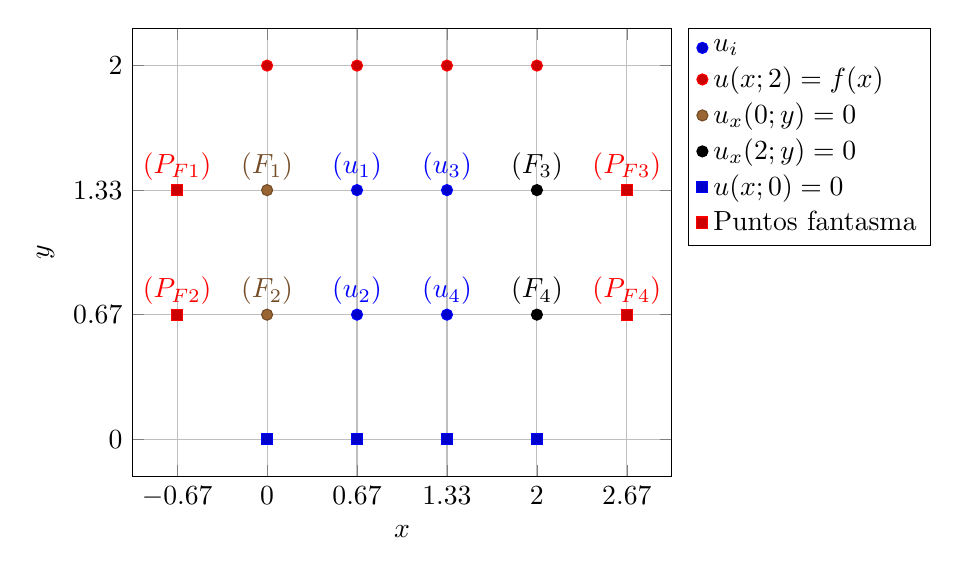
\begin{tikzpicture}
\begin{axis}[grid,xtick distance=2/3,ytick distance=2/3,legend cell align=left,
legend pos=outer north east,nodes near coords,enlargelimits=0.1,xmin=-2/3,xmax=8/3]

\addplot+[only marks,
point meta=explicit symbolic]
coordinates {
    (2/3,2/3) [($u_2$)]
    (4/3,2/3) [($u_4$)]

    (2/3,4/3) [($u_1$)]
    (4/3,4/3) [($u_3$)]
};
\addplot+[only marks,mark=*,
point meta=explicit symbolic]
coordinates{
    (0,2)
    (2/3,2)
    (4/3,2)
    (2,2)
};

\addplot+[only marks,mark=*,
point meta=explicit symbolic]
coordinates{
    (0,4/3) [($F_1$)]
    (0,2/3) [($F_2$)]
};
\addplot+[only marks,mark=*,
point meta=explicit symbolic]
coordinates{
    (2,4/3) [($F_3$)]
    (2,2/3) [($F_4$)]
};
\addplot+[only marks,mark=square*,
point meta=explicit symbolic]
coordinates{
    (0,0)
    (2/3,0)
    (4/3,0)
    (2,0)
};
\addplot+[only marks,mark=square*,
point meta=explicit symbolic]
coordinates{
    (-2/3,2/3) [($P_{F2}$)]
    (-2/3,4/3) [($P_{F1}$)]
    (8/3,2/3) [($P_{F4}$)]
    (8/3,4/3) [($P_{F3}$)]
};
\legend{$u_i$,$u(x;2)=f(x)$,$u_x(0;y)=0$,$u_x(2;y)=0$,$u(x;0)=0$,Puntos fantasma}
\end{axis}
\end{tikzpicture}

\end{document}